\section{Theory of high-resolution methods}

The above Godunov methods are at most first order accurate.
To achieve high-resolution methods we need to understand the structure of finite volume (FV) methods better.
We consider again only scalar equations.


\subsection{Structure of FV methods}

\begin{definition}[Structure of FV methods]
	Let \(u_j^{n + 1} = H_{\Delta t}\parentheses*{u_{\Delta x}^n; j}\) be a time-step method.
	The method \(H_{\Delta t}\) is called
	\begin{enumerate}
		\item \emph{monotone}, if for two solutions \(u_j^n\) and \(v_j^n\)
		\[
			u_j^n \le v_j^n \implies H_{\Delta t}\parentheses*{u_{\Delta x}^n; j} \le H_{\Delta t}\parentheses*{v_{\Delta x}^n; j} \quad \forall j \in \text{grid},
		\]
		\item \emph{\(L^1\)-contracting}, if
		\[
			\norm*{H_{\Delta t}\parentheses*{u_{\Delta x}^n; \cdot} - H_{\Delta t}\parentheses*{v_{\Delta x}^n; \cdot}}_1 \le \norm*{u_{\Delta x}^n - v_{\Delta x}^n}_1 \equiv \norm*{u_{\Delta t}\parentheses*{\cdot, t_n} - v_{\Delta t}\parentheses*{\cdot, t_n}}_1,
		\]
		\item \emph{total-variation-diminishing (TVD)}, if
		\[
			TV\parentheses*{u_{\Delta t}\parentheses*{\cdot, t_{n + 1}}} \equiv TV\parentheses*{u_{\Delta x}^{n + 1}} \le TV\parentheses*{u_{\Delta x}^n} \equiv TV\parentheses*{u_{\Delta t}\parentheses*{\cdot, t_n}},
		\]
		\item \emph{monotonicity-preserving}, if
		\[
			u_j^n \le u_{j + 1}^n \implies H_{\Delta t}\parentheses*{u_{\Delta x}^n; j} \le H_{\Delta t}\parentheses*{u_{\Delta x}^n; j + 1} \quad \forall j \in \text{grid}.
		\]
	\end{enumerate}
\end{definition}

\begin{remark}
	\begin{enumerate}
		\item We already saw these kind of definitions and properties in the context of Kruzkov's theorem.
		We would like to copy this to the numerical level.
		\item For a piecewise constant grid function \(u_{\Delta t}\) at time \(t_n\) we have
		\[
			TV\parentheses*{u_{\Delta x}^n} = \sum_{j \in \text{grid}}\absolute*{u_{j + 1}^n - u_j^n}.
		\]
		\item In the next section we will prove the following picture, where the entire box represents all FV methods.
		\begin{center}
			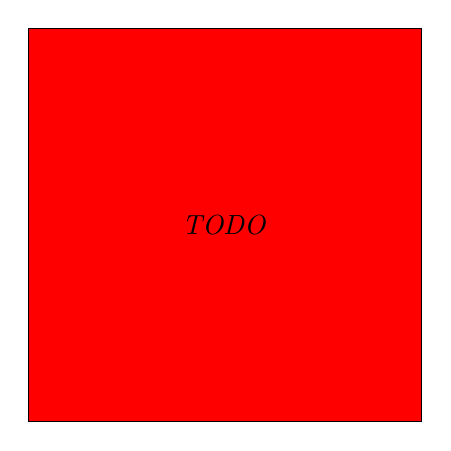
\begin{tikzpicture}
				\filldraw[fill=red] (0,0) rectangle (5,5) node[pos=.5] {\emph{TODO}};
			\end{tikzpicture}
		\end{center}
	\end{enumerate}
\end{remark}


\subsection{From monotone to monotonicity-preserving}

\begin{theorem}[Structure of FV methods]
	For a time-step method \(H_{\Delta t}\) in conservative form with \(3\)-point-stencil \(u_j^{n + 1} = H_{\Delta t}\parentheses*{u_{j - 1}^n, u_j^n, u_{j + 1}^n; j}\), the following implications hold for the method \(H_{\Delta t}\):
	\[
		\text{monotone} \xrightarrow{\text{(i)}} L^1\text{-contracting} \xrightarrow{\text{(ii)}} \text{TVD} \xrightarrow{\text{(iii)}} \text{monotonicity-preserving}.
	\]
\end{theorem}

\begin{proof}
	
\end{proof}

\begin{theorem}[Monotone methods]
	A monotone FV method \(u_j^{n + 1} = H_{\Delta t}\parentheses*{u_{j - 1}^n, u_j^n, u_{j + 1}^n; j}\) for a scalar conservation law is at most first order \emph{accurate} (i.e., order \(1\) convergent).
\end{theorem}

\begin{proof}
	
\end{proof}

\subsection{Theorem of Godunov}

\begin{theorem}[Godunov]
	A linear, monotonicity-preserving method is at most first order accurate.
\end{theorem}

\begin{proof}
	
\end{proof}

\begin{remark}
	\begin{enumerate}
		\item Monotonicity-preservation is essential to avoid the generation of oscillations at discontinuities.
		According to the theorem it is only possible to obtain higher order of convergence with nonlinear methods.
		\item In a nonlinear method a linear method is typically modified such that the method coefficients depend additionally on the solution itself and can change accordingliy.
	\end{enumerate}
\end{remark}

\begin{example}[Monotone and non-monotone methods]
	
\end{example}


\subsection{Convergence of TVD-methods}

For linear methods we have build convergence on the stability statement of the form
\[
	\norm*{u_{\Delta x}^{n + 1}} \le C\norm*{u_{\Delta x}^n},
\]
using an appropriate norm.
For nonlinear methods this stability will be replaced by a total-variation-diminishing property
\[
	TV\parentheses*{u_{\Delta x}^{n + 1}} \le TV\parentheses*{u_{\Delta x}^n},
\]
which leads to so-called \emph{total-variation-diminishing (TVD) methods}.
We will do this for a conservation on a finite time horizon.

\begin{theorem}[Convergence of finite-volume methods]
	Consider the scalar conservation law
	\[
		\partial_t u + \partial_x f\parentheses*{u}, \quad \parentheses*{x, t} \in \R \times \brackets*{0, T}, \qquad u\parentheses*{x, 0} = u_0\parentheses*{x}, \quad x \in \R
	\]
	for some \(T > 0\).
	Suppose its solution is approximated by a TVD-method in conservative form based on a consistent and Lipschitz-continuous, numerical flux.
	Suppose further that the initial conditions satisfies \(TV\parentheses*{u_0} \le C\) and let \(u_{\Delta t}^{\parentheses*{T}}: \R \times \brackets*{0, T} \to \R\) be the piecewise constant numerical grid function based on the grid size \(\Delta x\) (recall \(\frac{\Delta x}{\Delta t} = \text{const.}\)) using all time levels.
	The sequence
	\[
		\braces*{u_{\Delta t_k}^{\parentheses*{T}}}_{k \in \N}\text{ with }\Delta t_k \xrightarrow{t \to \infty} 0
	\]
	converges (possibly after selection of a sub-sequence) in the \(L^1\parentheses*{\R \times \brackets*{0, T}}\)-norm to a weak solution \(u: \R \times \brackets*{0, T} \to \R\) of the conservation law.
\end{theorem}

\begin{remark}
	
\end{remark}


\subsection{Compactness}

As mentioned in the previous remark, we may only be able to assure convergence along subsequences.
To ensure the existence of convergent subsequences, we first need the following concept.

\begin{definition}[Compactness]
	A set \(M\) is called \emph{compact}, if for every sequence \(\braces*{g_k}_{k \in \N} \subset M\) there exists a subsequence
	\[
		\braces*{g_{\ell_k}}_{k \in \N} \quad \text{(with }\braces*{\ell_k}_{k = 1, 2, \ldots}\text{strictly increasing numbers)}
	\]
	which is convergent in \(M\)
\end{definition}

\begin{example}[Compactness]
	
\end{example}

The following result then provides a condition for the existence of convergent subsequences,
which is convenient for our discussion.

\begin{theorem}[Compactness in BV]
	
\end{theorem}